\chapter{Lec 11 - Higher-order functions using fold}

\section{Map and filter functions using fold-left}
The fold function can be seen as a polymorphic generalization of the foreach statement. So, we can try to write the \textbf{map} function using fold-left.\newline\newline
The fold-left function is defined as follows:
\begin{lstlisting}[style = FSharpStyle]
    let rec foldL f z l =
    match l with
    | [] -> z
    | x :: xs -> foldL f (f z x) xs

    //Type : val foldL : f:('a -> 'b -> 'a) -> z:'a -> l:'b list -> 'a
\end{lstlisting}
The map function creates a new list transforming each element of the input list into another element according to a function $f$.\newline\newline
An implementation of the map function using fold-left can be the follow:
\begin{lstlisting}[style = FSharpStyle]
    let map f l = foldL (fun z x -> z @ [f x]) [] l
    map (fun x -> x*x) [1..5]

    //Result: int list = [1; 4; 9; 16; 25]

    let map2 f l = foldL (fun z x -> f x :: z) [] l
    map2 (fun x -> x*x)[1..5]

    //Result: int list = [25; 16; 9; 4; 1]
\end{lstlisting}
The code above defines two implementations of the map function. The behavior of the two functions is to map each number to its respective square. The fold-left function consents to store the squares list in the accumulator and to forward it to the next recursive step. At the end, the accumulator will contain the mapped list to return. As you can see, the results are slightly different (one list is the reverse of the other). This is due to how the list to pass as accumulator is generated. 
\begin{itemize}
    \item In the first case, at each recursive step, the accumulator is forwarded according to the following expression:
    \begin{lstlisting}[style = FSharpStyle]
    z @ [f x]
    \end{lstlisting}
    The $@$ operator takes two lists and produces a new list, basically it \textit{concatenates} two lists. So, in this case we can concatenate the result of the application of \textbf{f} on the current element \textbf{x} (using the temporary list [f x]) to the content of the accumulator. Basically, the accumulator is forwarded to the next step by "\textit{adding}"\footnote{Note that is not an actual adding operation since we are creating a new list, at each step, with the mapped element in last position} the mapped element [f x] at the \textbf{end} of the list contained in the accumulator at the previous step. By doing this, the resulting list will be in the same order as the input list.
    \begin{lstlisting}[style = FSharpStyle]
    [] + [1] = [1]
    [1] + [4] = [1; 4]
    [1; 4] + [9] = [1; 4; 9]
    [1; 4; 9] + [16] = [1; 4; 9; 16]
    [1; 4; 9; 16] + [25] = [1; 4; 9; 16; 25]
    \end{lstlisting}

    \item In the second function, instead, the accumulator is forwarded according to this expression:
    \begin{lstlisting}[style = FSharpStyle]
    f x :: z
    \end{lstlisting}
    The :: operator takes an \textbf{element} and a list and produces a list. It forwards the accumulator by creating a new list with the mapped element f x as head and the accumulator of the previous step as tail. So, since we are traversing the list \textit{from left to right}, the resulting list will be in the opposite order as the input list.
    \begin{lstlisting}[style = FSharpStyle]
    1 + [] = [1]
    4 + [1] = [4; 1]
    9 + [4; 1] = [9; 4; 1]
    16 + [9; 4; 1] = [16; 9; 4; 1]
    25 + [16; 9; 4; 1] = [25; 16; 9; 4; 1]
    \end{lstlisting}
    \end{itemize}
    Note that we can't pattern-match on the @ operator because it is just a function and not a data constructor.\newline\newline
    Implementing the map function using fold-right instead of fold-left would lead to the opposite result (the resulting list using :: operator will be in the \textit{correct} order and the resulting list using @ will be reversed).\newline\newline
    The same approach can be followed in order to write the \textbf{filter} function.
    \begin{lstlisting}[style = FSharpStyle]
        let filter f l = foldL (fun z x -> if f x then z @ [x] else z) [] l
        filter (fun x -> x > 10) [1..20]

        //Result: [11; 12; 13; 14; 15; 16; 17; 18; 19; 20]

        let filter2 f l = foldL (fun z x -> if f x then x :: z else z) [] l
        filter2 (fun x -> x > 10) [1..20]

        //Result: [20; 19; 18; 17; 16; 15; 14; 13; 12; 11]
    \end{lstlisting}
    All the methods presented until now are provided in the List module of the F\# standard library.
    \section{Max function}
    The \textbf{max} function defined in the List module of the F\# standard library has the following type
    \begin{center}
        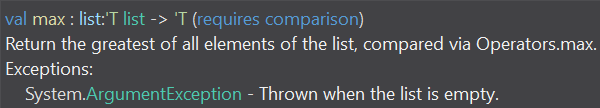
\includegraphics[]{images/MAx type.png}
    \end{center}
    The type 'T requires a \textbf{comparison} constraint. It means that the max function works correctly as long as the type 'T implements the $<$ operator (less than). F\# consents you to add constraints to types, but if we don't want to use this advanced feature and we want to write the max function from scratch, we need to pass an additional function as parameter that performs the comparison. Also this kind of function is already defined in the List module and is called \textbf{maxBy}.\newline\newline
    An implementation of the maxBy function can be the following:
    \begin{lstlisting}[style = FSharpStyle]
        let rec max_by cmp l =
            match l with
            | [] -> raise (Failure "message")
            | [x] -> x
            | x::xs -> let m = max_by cmp xs in if cmp x m then m else x

        //Type: val max_by : cmp:('a -> 'a -> bool) -> l:'a list -> 'a

        max_by (<) [1; -33; 55; 1]

        //Result: val it : int = 55
    \end{lstlisting}
    If the list is empty it raises an exception. Otherwise, it recursively goes at the end of the list and select the last element as maximum. Ascending from the recursion it compares each element with the current maximum. If the current element \textbf{x} is greater than the maximum, this element becomes the maximum. At the end, the function returns the max value of the input list. Writing the function this way avoids adding an extra parameter in which to store the current maximum value.\newline\newline
    The \textbf{in} keyword separates what you want to do after a binding. If you write the expression after the binding on a new line you don't need this keyword.
    \subsection{MaxBy function using fold-left}
    MaxBy function can be defined also using the fold-left function by storing in the accumulator the current maximum value. The problem is how to set the initial value of the accumulator, because the initial max value is \textbf{unknown}. To express the concept of unknown value in F\# we can use \textbf{option type}
    \begin{lstlisting}[style = FSharpStyle]
        type 'a option = None | Some of 'a
    \end{lstlisting}
    The type 'a can be either None or Something of type 'a\footnote{As usual, this type is already defined in the F\# standard library}.\newline\newline
    Now we can implement maxBy using fold-left as follows:
    \begin{lstlisting}[style = FSharpStyle]
        let max_by_fold cmp l=
            let f m x = 
                match m with
                | None -> Some x
                | Some y -> if cmp x y then Some y else Some x
            foldL f None l

        //Type: val max_by_fold : cmp:('a -> 'a -> bool) -> l:'a list -> 'a option 
        
        max_by_fold (<) [1; -33; 55; 100] 

        //Result: Some 100
    \end{lstlisting}
    This implementation works by defining a \textbf{nested} function \textbf{f} that performs the comparison between the element \textbf{x} and the current max value (taking into account the fact that the type of the accumulator is \textit{'a option}). Then this function is passed to foldL with the initial state of the accumulator equals to None. 

